\section{Appendix}\label{section:appendix}

The figures in this appendix supplement those in the main text. Figures already shown in the Results section are not repeated here.

\subsection*{VQE Algorithm}

\Cref{alg:vqe} gives a self-contained description of the VQE procedure as implemented in this project. All source code is available in the project repository \parencite{fys5419-repo}.

\begin{algorithm}[H]
\caption{Variational Quantum Eigensolver (VQE)}
\label{alg:vqe}
\begin{algorithmic}[1]
\Require Hamiltonian $\mathcal{H} = \sum_k c_k P_k$, ansatz $U(\boldsymbol{\theta})$, initial parameters $\boldsymbol{\theta}_0$
\Ensure Approximate ground state energy $E_{\mathrm{VQE}}$
\State Decompose $\mathcal{H}$ into Pauli strings $\{P_k\}$ with real coefficients $\{c_k\}$
\State Initialize $\boldsymbol{\theta} \leftarrow \boldsymbol{\theta}_0$
\Repeat
  \State Prepare trial state $\ket{\psi(\boldsymbol{\theta})} = U(\boldsymbol{\theta})\ket{0}^{\otimes n}$
  \For{each Pauli term $P_k$}
    \State Rotate to the appropriate measurement basis
    \State Evaluate expectation value $\langle P_k \rangle_{\boldsymbol{\theta}}$
  \EndFor
  \State Compute energy $E(\boldsymbol{\theta}) = \sum_k c_k \langle P_k \rangle_{\boldsymbol{\theta}}$
  \State Update $\boldsymbol{\theta}$ via classical optimizer (BFGS / L-BFGS-B)
\Until{$|E(\boldsymbol{\theta}_{t+1}) - E(\boldsymbol{\theta}_t)| < \epsilon_{\mathrm{tol}}$}
\State \Return $E_{\mathrm{VQE}} = E(\boldsymbol{\theta}^{\ast})$
\end{algorithmic}
\end{algorithm}

% ---------- Part C (supplementary) ----------
\subsection*{Part C: Additional VQE diagnostics for the two-level model}

\begin{figure}[H]
\centering
\begin{subfigure}[t]{0.4\textwidth}
\centering
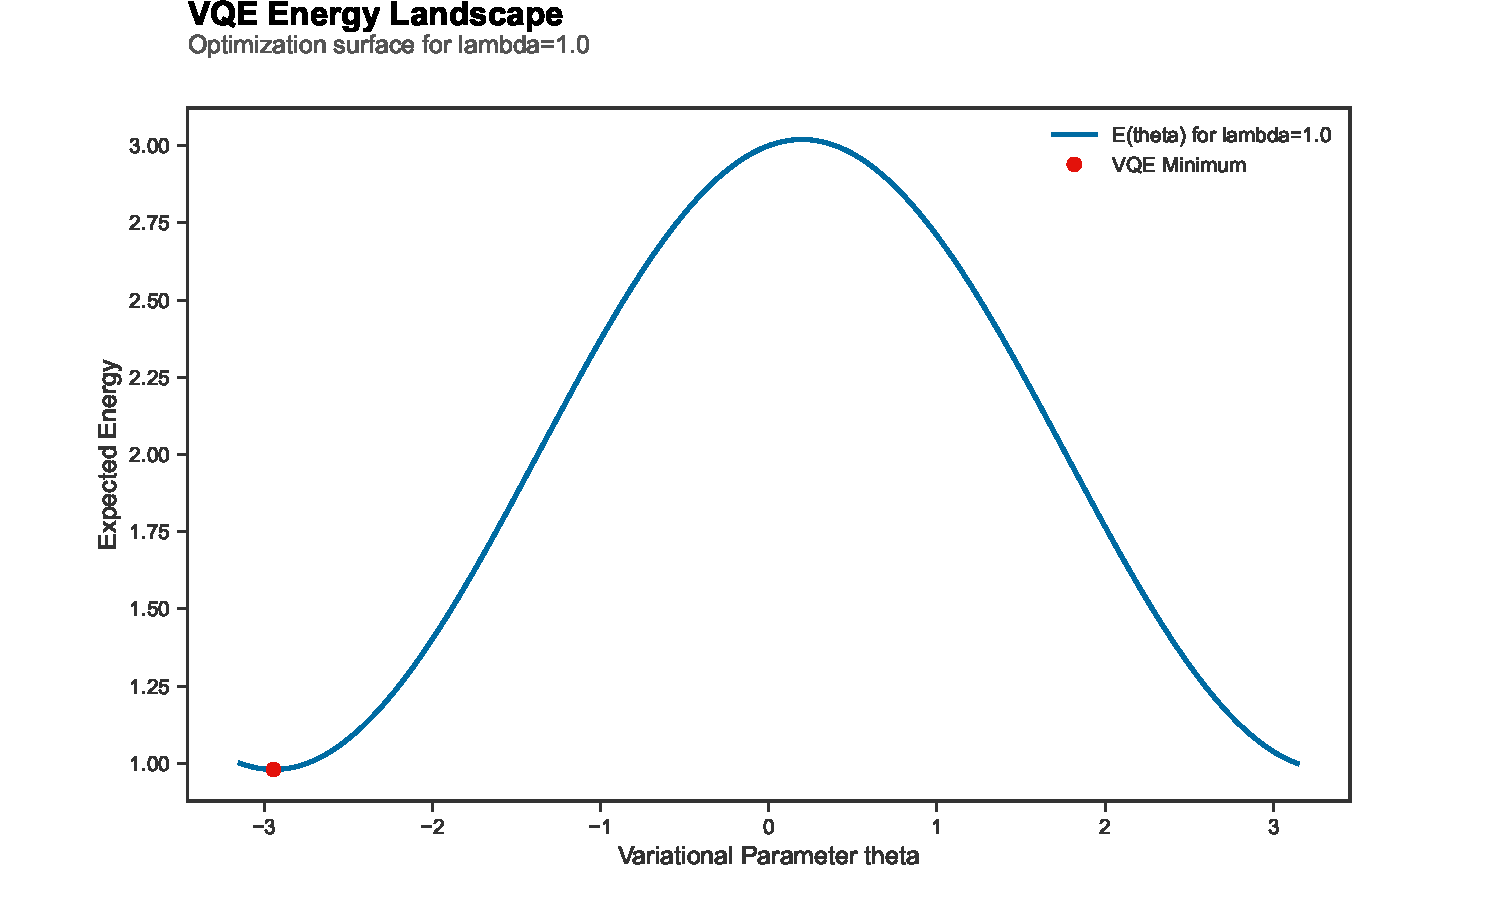
\includegraphics[width=\linewidth]{figures/part-c_energy_landscape.pdf}
\caption{Energy landscape $E(\theta)$ for the $R_y$ ansatz at selected values of $\lambda$, showing the smooth, unimodal structure that ensures reliable BFGS convergence.}
\label{fig:app_c_landscape}
\end{subfigure}
\hfill
\begin{subfigure}[t]{0.4\textwidth}
\centering
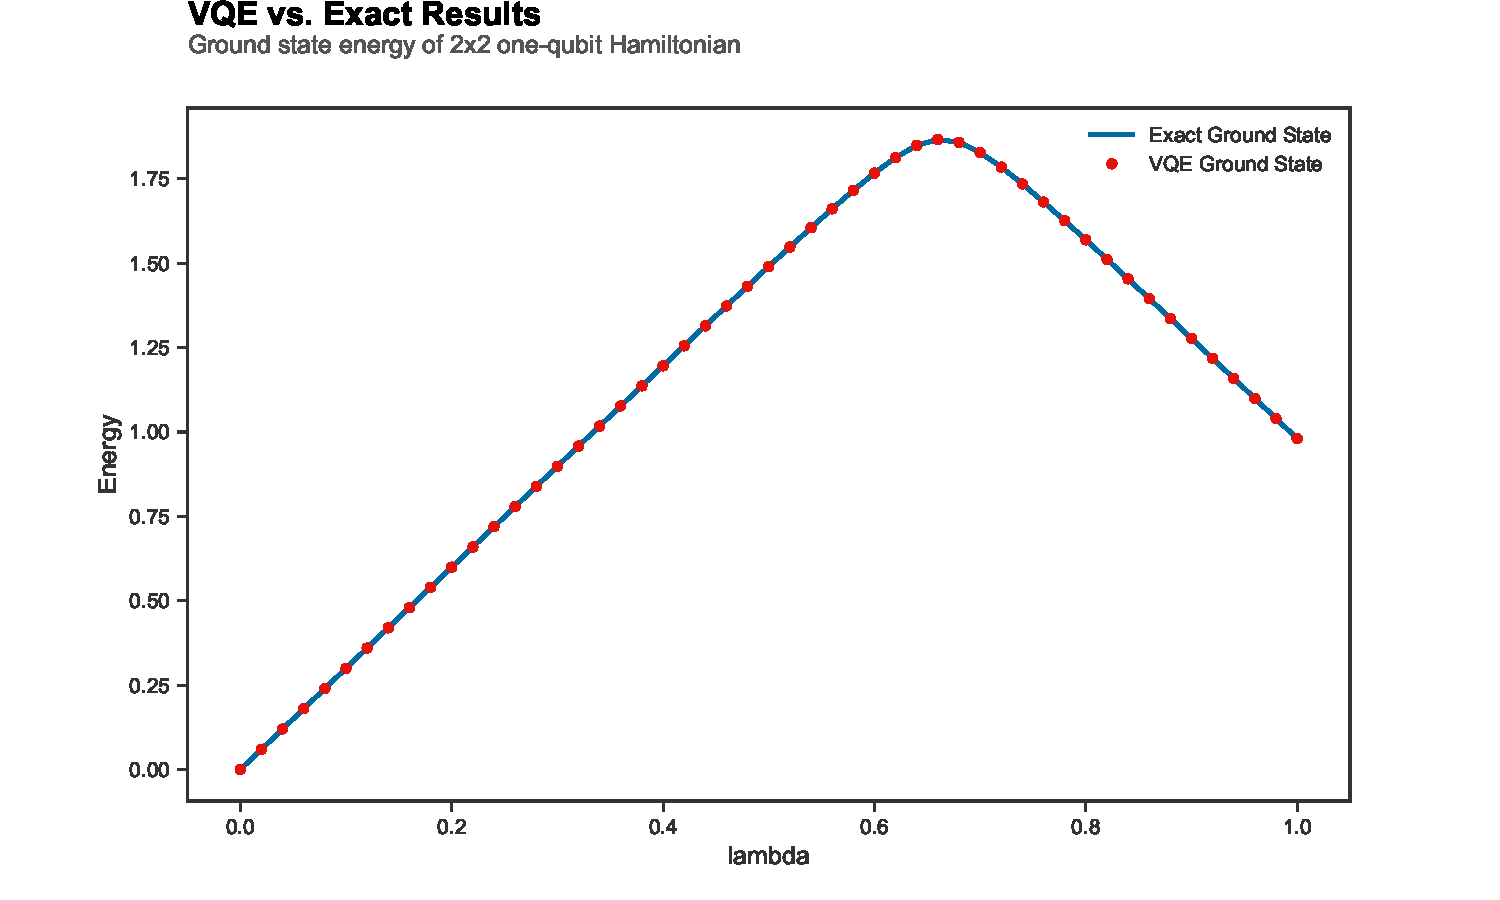
\includegraphics[width=\linewidth]{figures/part-c_vqe_comp.pdf}
\caption{VQE ground state energy vs.\ exact diagonalization across $\lambda\in[0,1]$.}
\label{fig:app_c_comp}
\end{subfigure}

\vspace{0.6em}

\begin{subfigure}[t]{0.4\textwidth}
\centering
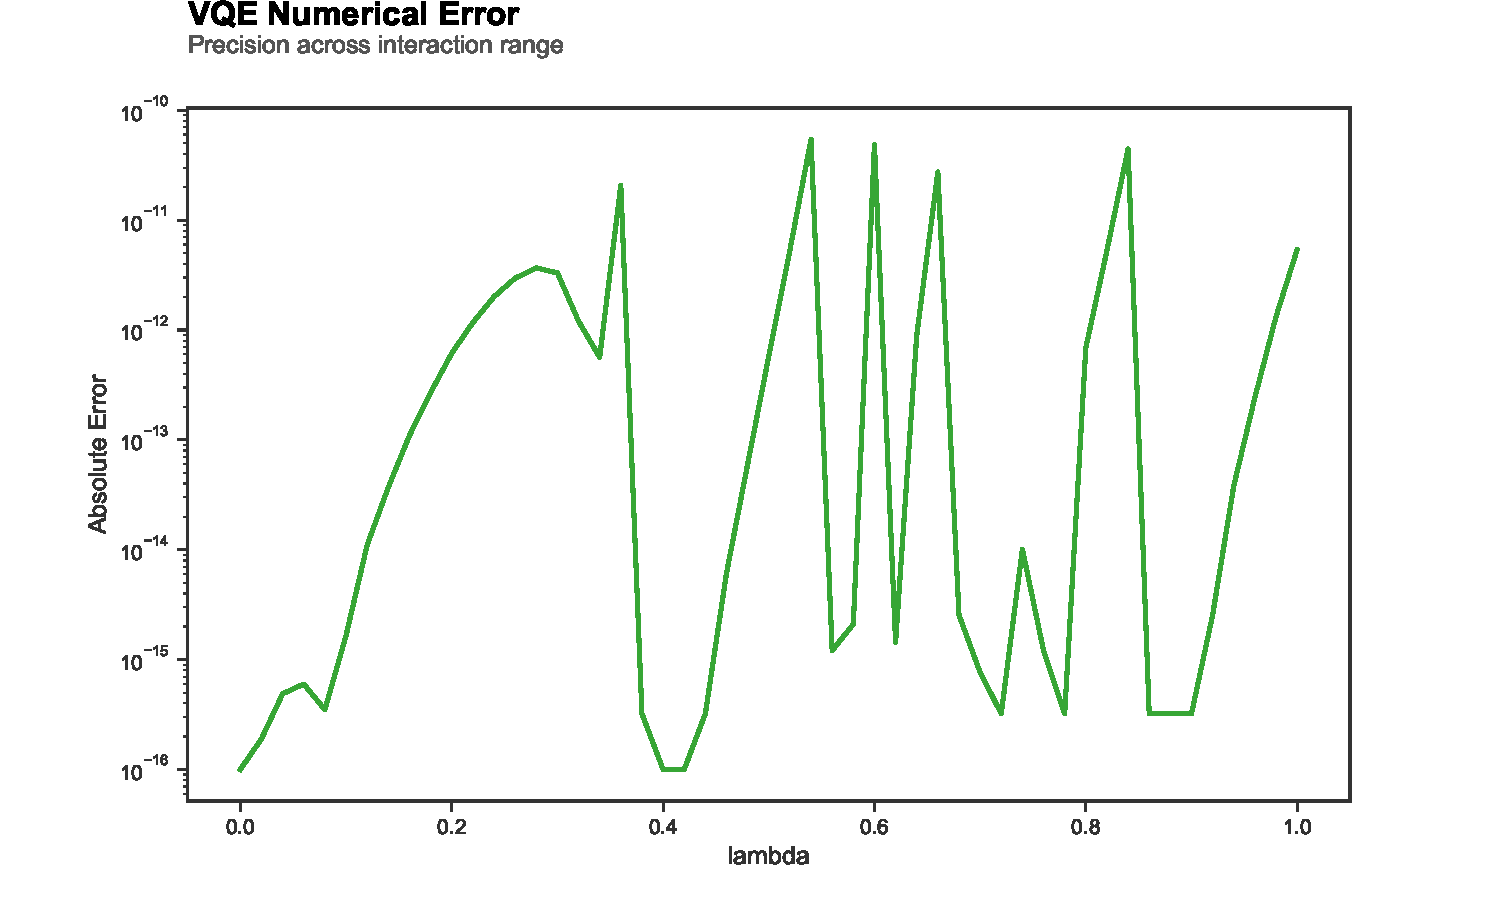
\includegraphics[width=\linewidth]{figures/part-c_vqe_error.pdf}
\caption{Absolute VQE error as a function of $\lambda$ for the single-qubit model.}
\label{fig:app_c_err}
\end{subfigure}
\hfill
\begin{subfigure}[t]{0.4\textwidth}
\centering
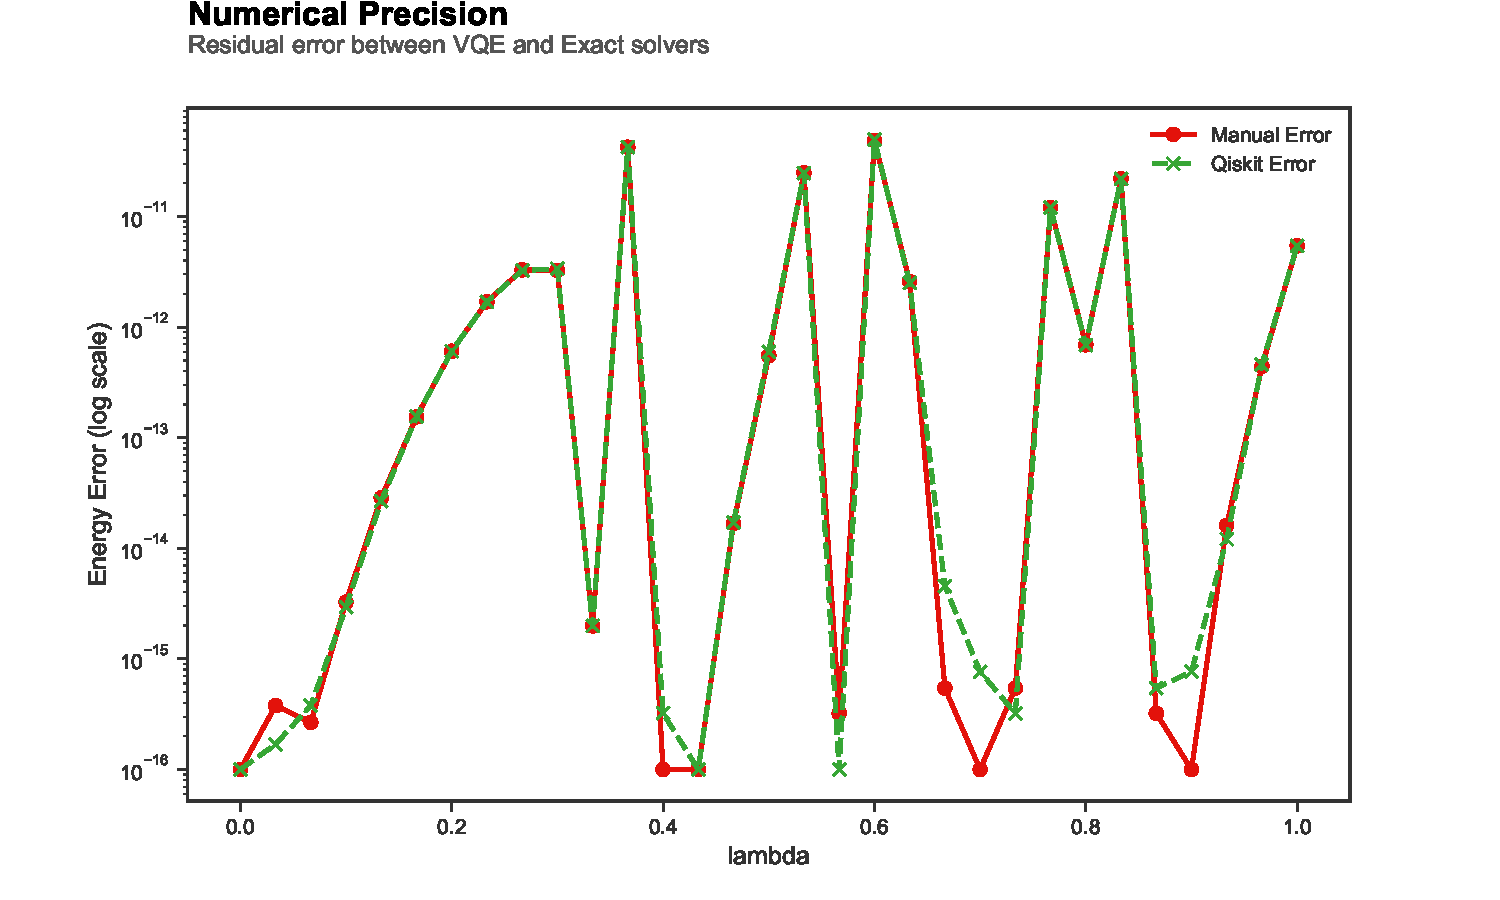
\includegraphics[width=\linewidth]{figures/part-c_vqe_precision.pdf}
\caption{Log-scale precision plot showing error remaining below $10^{-10}$ throughout.}
\label{fig:app_c_prec}
\end{subfigure}

\vspace{0.6em}

\begin{subfigure}[t]{0.4\textwidth}
\centering
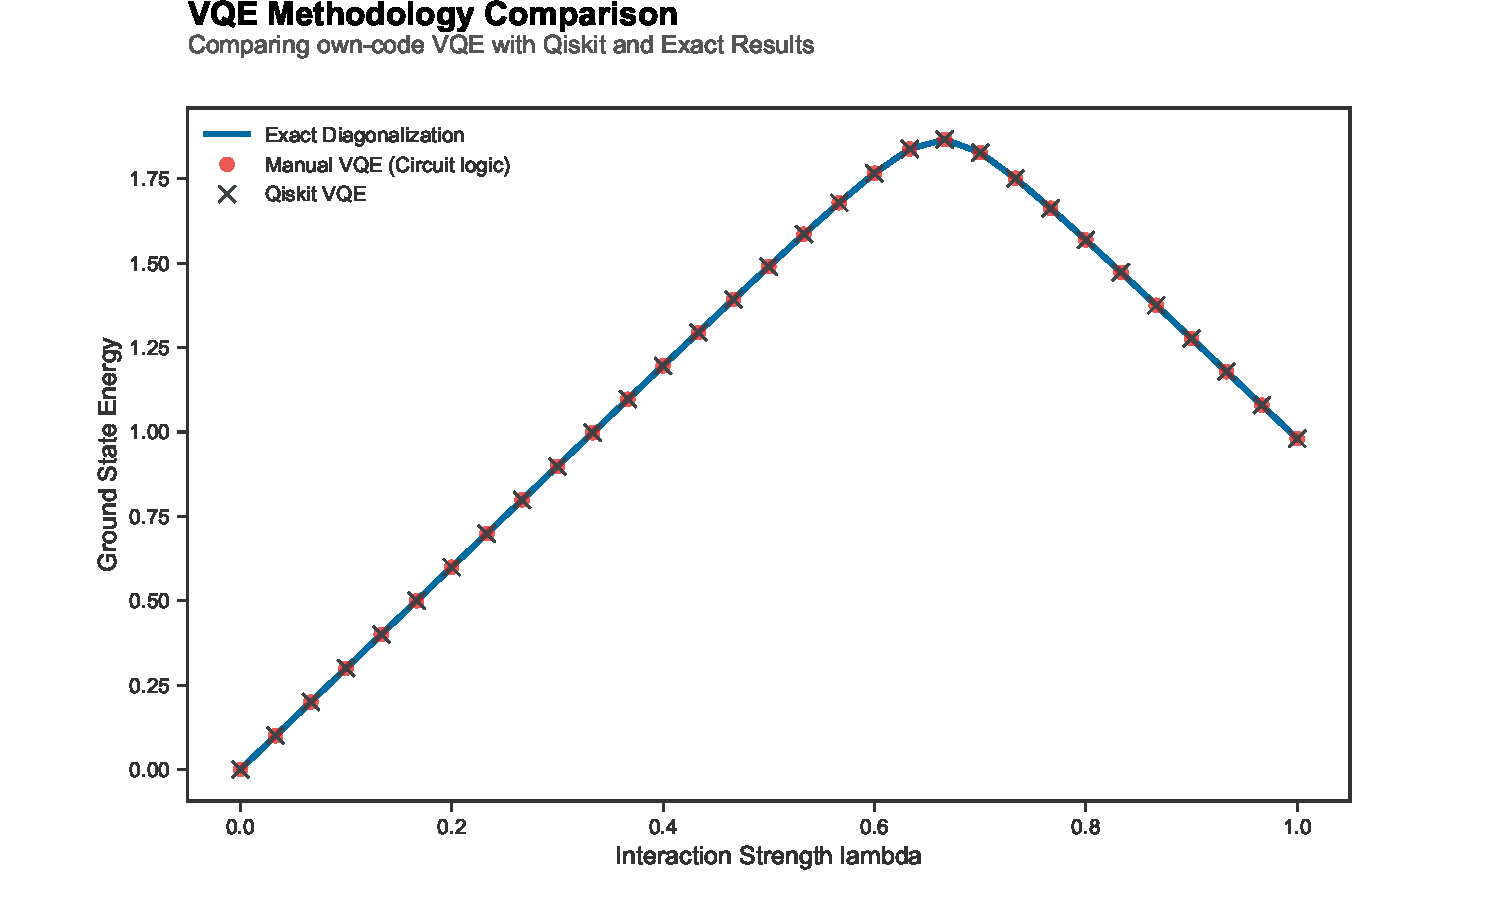
\includegraphics[width=\linewidth]{figures/part-c_vqe_method_comparison.pdf}
\caption{Comparison between manual VQE implementation and Qiskit \texttt{SparsePauliOp} for the two-level model.}
\label{fig:app_c_methods}
\end{subfigure}
\caption{Supplementary VQE diagnostics for the $2\times2$ two-level Hamiltonian (Part c).}
\label{fig:app_c}
\end{figure}

% ---------- Part E (supplementary) ----------
\subsection*{Part E: Additional VQE diagnostics for the two-qubit model}

\begin{figure}[H]
\centering
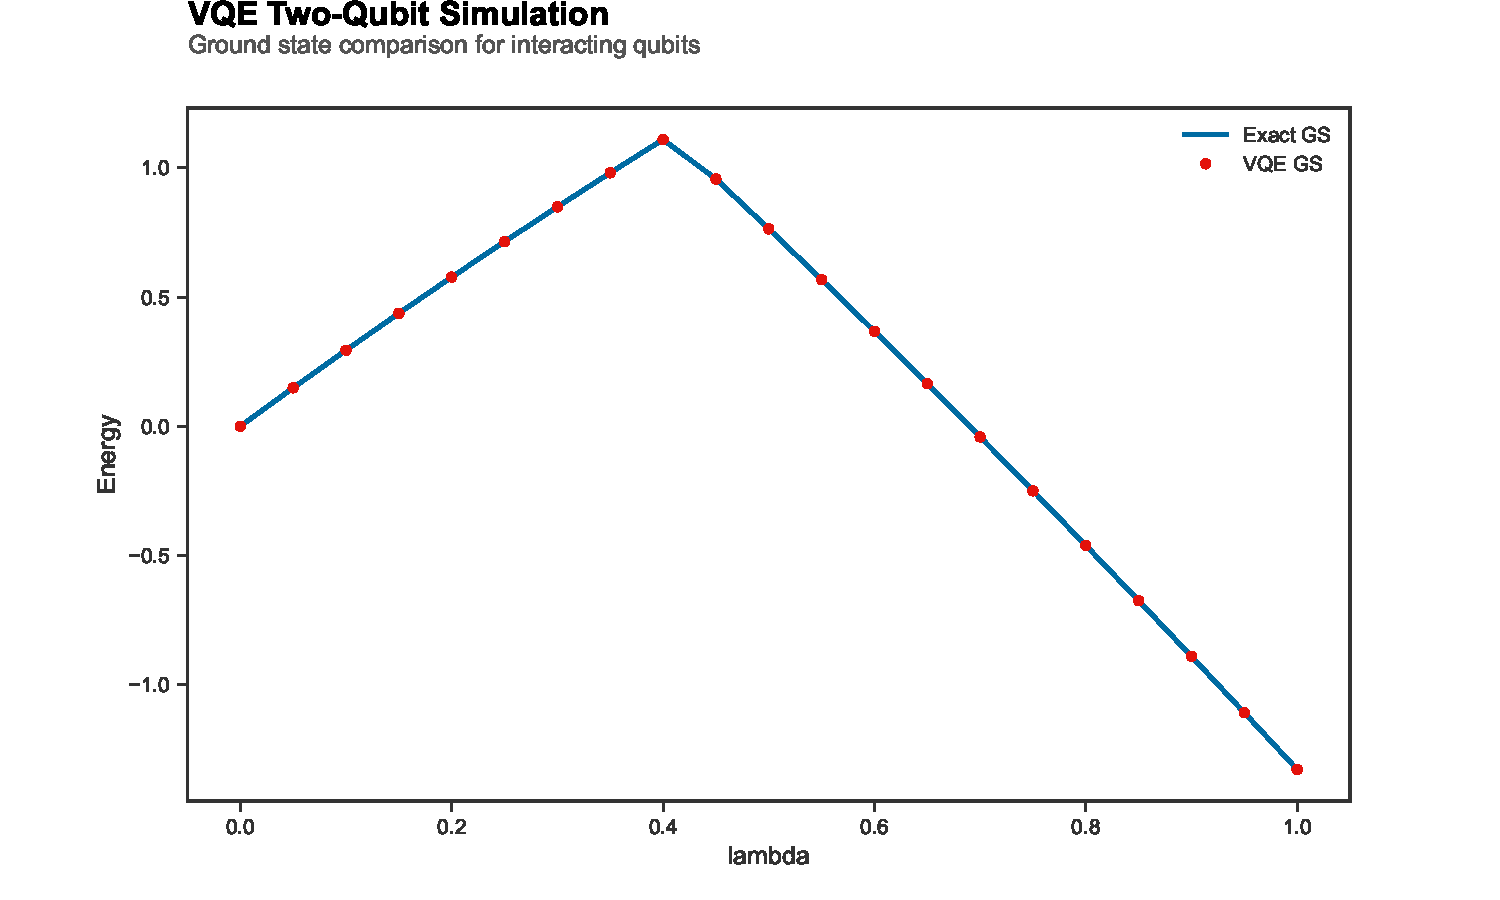
\includegraphics[width=0.48\textwidth]{figures/part-e_vqe_comp.pdf}
\caption{VQE ground state energy vs.\ exact diagonalization for the two-qubit Hamiltonian, showing agreement across the full $\lambda$ range.}
\label{fig:app_e_comp}
\end{figure}

% ---------- Part G (supplementary) ----------
\subsection*{Part G: Additional Lipkin VQE diagnostics}

\begin{figure}[H]
\centering
\begin{subfigure}[t]{0.4\textwidth}
\centering
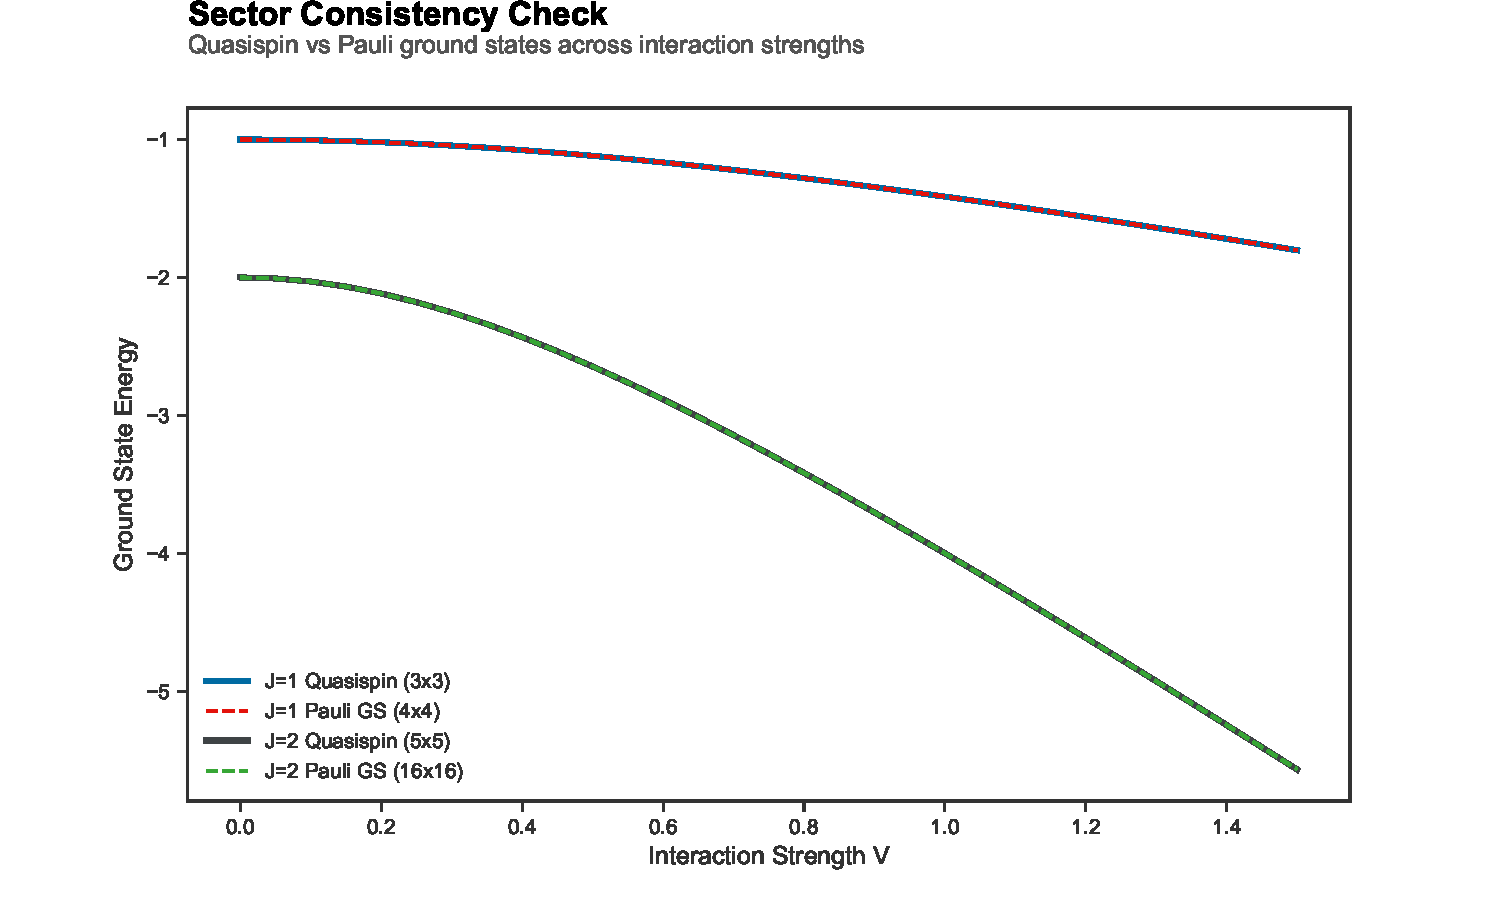
\includegraphics[width=\linewidth]{figures/part-g_sector_check.pdf}
\caption{Verification that the VQE correctly identifies eigenvalues within the $J=2$ sector of the full $16\times16$ qubit Hilbert space, matching the quasispin reference values.}
\label{fig:app_g_sector}
\end{subfigure}
\hfill
\begin{subfigure}[t]{0.4\textwidth}
\centering
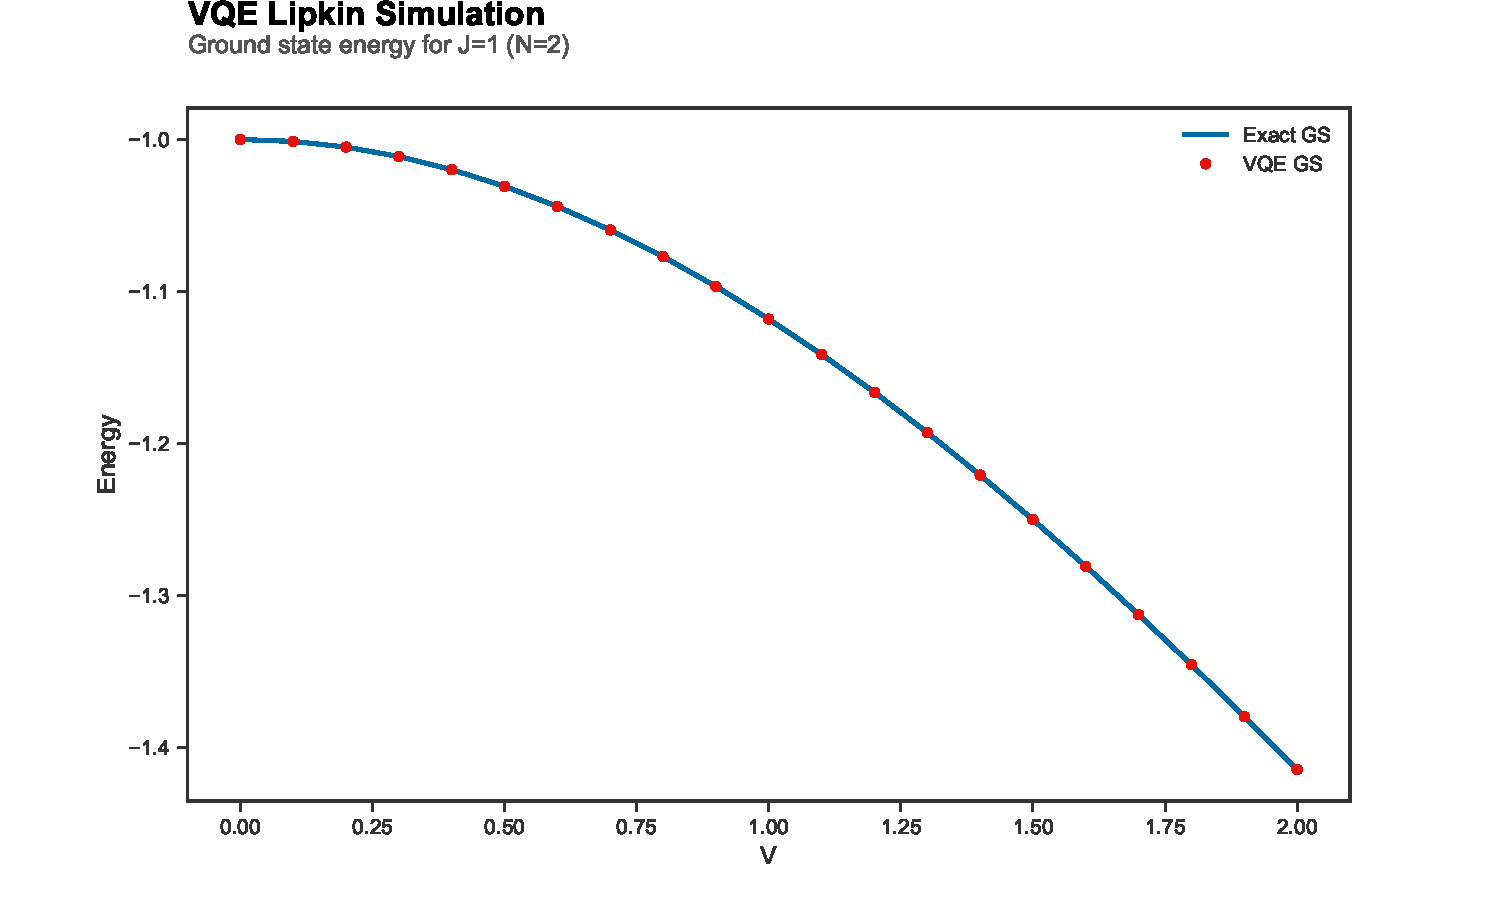
\includegraphics[width=\linewidth]{figures/part-g_vqe_j1.pdf}
\caption{VQE ground state energy for the Lipkin $J=1$ system as a function of $V$, with residual error at the $10^{-11}$ level.}
\label{fig:app_g_j1}
\end{subfigure}
\caption{Supplementary diagnostics for the Lipkin VQE (Part g).}
\label{fig:app_g}
\end{figure}


\subsection{Circuits}

\begin{figure}[H]
    \centering
    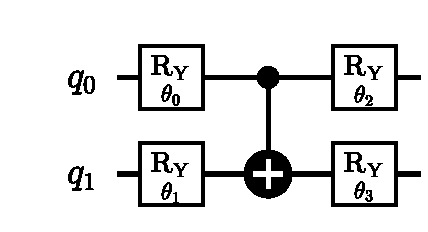
\includegraphics[width=0.45\textwidth]{figures/circuit_part_e.pdf}
    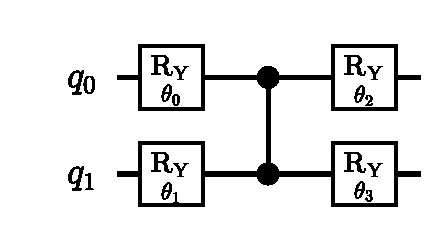
\includegraphics[width=0.45\textwidth]{figures/circuit_part_g_j1.pdf}
    \vspace{0.5em}
    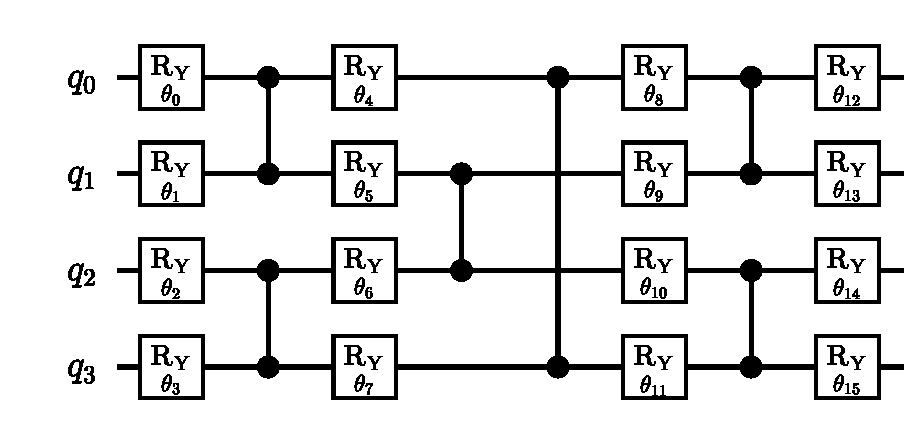
\includegraphics[width=0.9\textwidth]{figures/circuit_part_g_j2.pdf}
    
    \caption{Quantum circuits for all configurations.}
    \label{fig:circuits_appendix}
\end{figure}

% ---------- Python environment ----------
\subsection*{Python environment}

\begin{lstlisting}[
captionpos=b,
caption={Python environment and core libraries used for the numerical simulations, classical diagonalization, and quantum-circuit implementations in this project.},
label={lst:python-environment}
]
matplotlib>=3.7.1
numpy>=1.24.3
pandas>=2.2.2
pennylane>=0.38.0
qiskit>=1.0.0
qiskit-aer>=0.17.2
qiskit-algorithms>=0.4.0
scipy>=1.14.1
seaborn>=0.13.2
sympy>=1.13.3
\end{lstlisting}
